\section*{Lezione 5}
\addcontentsline{toc}{section}{Lezione 5}

\subsection*{Intepretazione geometrica}
\addcontentsline{toc}{subsection}{Interpretazione geometrica}
\subsubsection*{Cubi}
\addcontentsline{toc}{subsubsection}{Cubi}

Abbiamo detto che l'insieme $<\{0, 1\}^n, +_2, \cdot>$ è uno spazio vettoriale.
Supponiamo di avere $n=3$, quindi dal canale entrano ed escono vettori di 3 bit.
Diciamo che ognuno di questi bit rappresenta un lato di un cubo in tre dimensioni, successivamente "appoggiamo" questo cubo all'interno di uno spazio come ${\rm I\!R^3}$.

\begin{figure}[h]
	\centering
	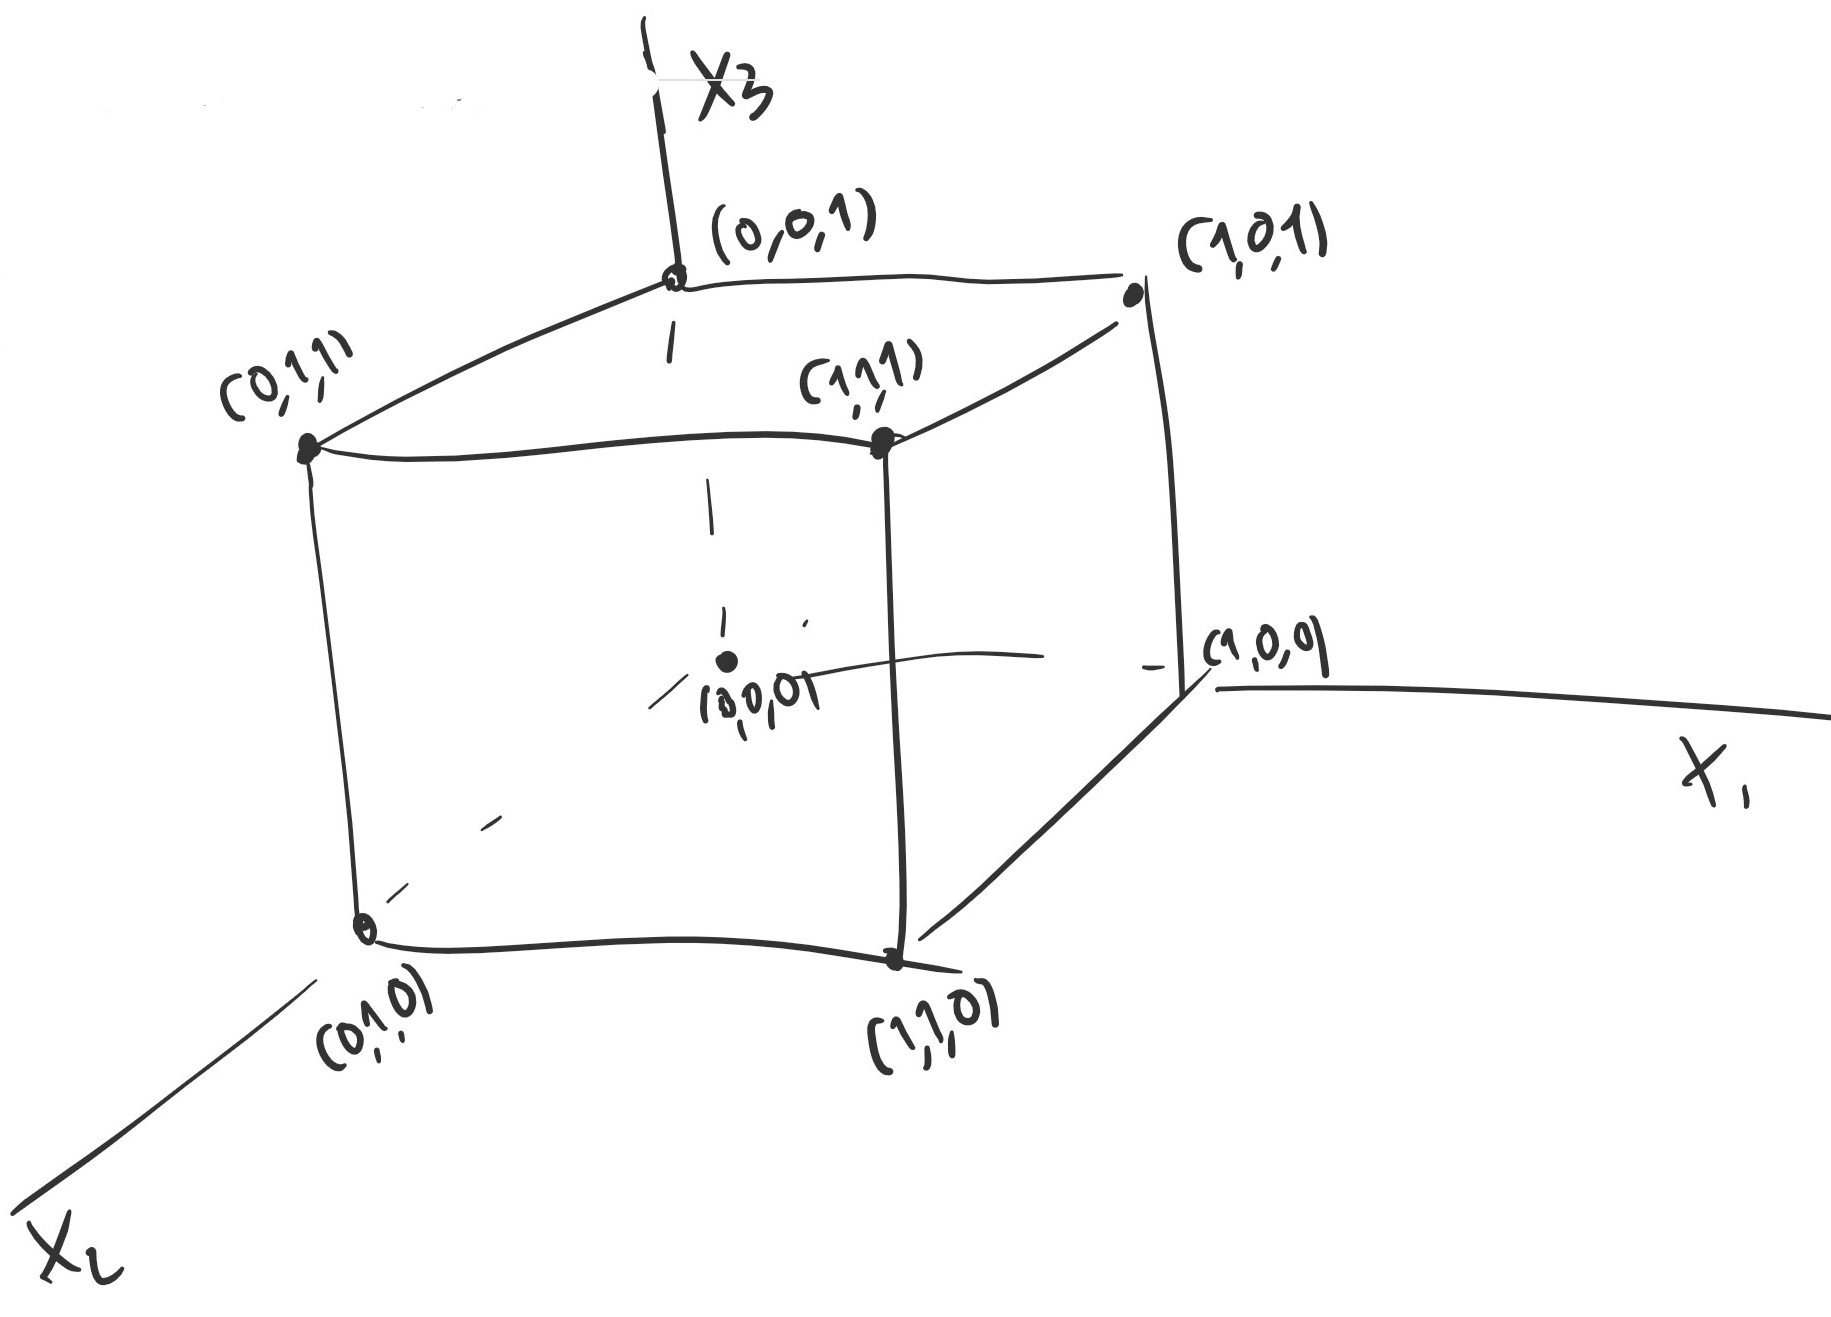
\includegraphics[width=0.7\linewidth]{immagini/img7}
\end{figure}

L'origine corrisponderà al messaggio (0, 0, 0), ogni asse rappresenterà quindi un bit.

L'idea è ovviamente utilizzabile in \textit{n} dimensione, usando quindi dei cubi di \textit{n} dimensioni.

I vertici del cubo rappresentano quindi tutte le possibile sequenze di messaggi. Un sottoinsieme di questi vettori, o vertici, rappresenta i messaggi "validi", quindi senza errore.
Ma cosa vuol dire dal punto di vista geometrico che un messaggio non è valido?
Supponiamo di mandare un messaggio 010, e che il rumore lo trasformi in 011. Un errore significa che ci siamo "mossi" da un vertice ad un altro del cubo. Un errore alla prima posizione ci fa muovere lungo l'asse $x_1$, un errore alla seconda posizione lungo l'asse $x_2$ e così via.

Il mittente e il destinatario devono quindi mettersi d'accordo su quali vertici siano "accettabili".

Mettiamo che i vertici accettabili siano 011 e 111

\begin{figure}[H]
	\centering
	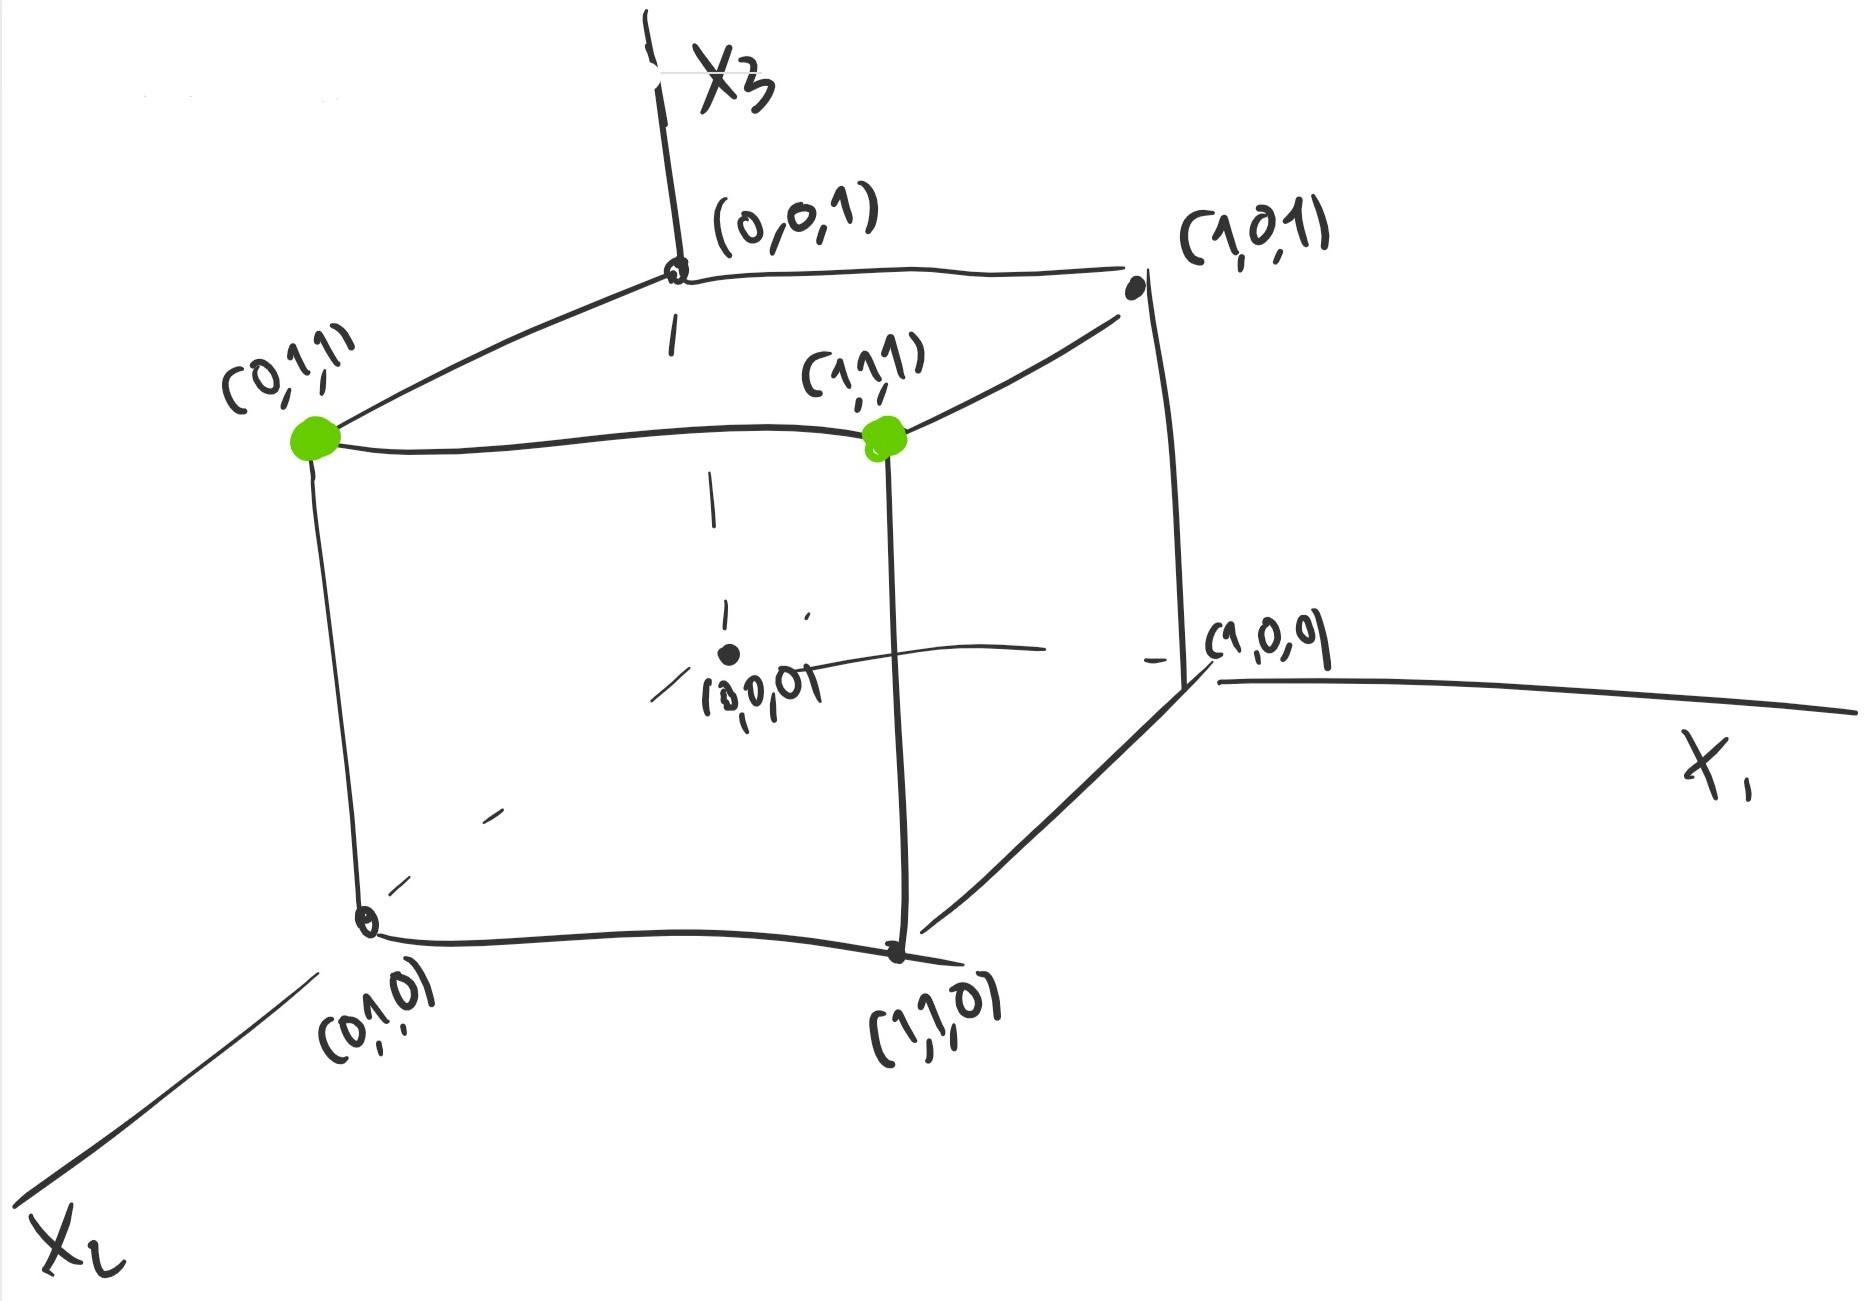
\includegraphics[width=0.7\linewidth]{immagini/img8}
\end{figure}


Ora mettiamo che nel canale il messaggio da 011 si sposti lungo la direzione $x_1$, quindi il messaggio diventa 111. Esso è accettabile però!

Definiamo la distanza di Hamming: dati due vettori \textit{u} e \textit{v} come il numero che bit che bisogna cambiare in \textit{u} per ottenere \textit{v} (e viceversa).

Ad esempio la distanza di Hamming fra 011 e 111 è 1.

Possiamo definire questa distanza anche usando la somma bit a bit.
$(0,1,1) \oplus (1,1,1) = (1,0,0)$
La distanza di Hamming è uguale a:
\begin{equation}
d_H(u)=\sum_{i=1}^{n}u_i
\end{equation}
Che rappresenta il numero di 1 all'interno dello xor bit a bit fra i due vettori.

Tornando al nostro cubo, diciamo che due vertici adiacenti non possono essere entrambi validi visto che, a causa di un errore, ci si sposta da uno all'altro; il mittente non rileverà l'errore!

Se nel mio codice la distanza di Hamming fra codici valdi è uguale a 1, non riuscirò mai a riconoscere errori.

Il numero di "passi" che devo fare da un vertice all'altro del cubo è uguale alla distanza di Hamming che c'è fra i due valori rappresentati dai vertici.

Se selezionassi le parole valide usando distanza di Hamming = 2?
Posso vedere la distanza fra i vertici in questo modo:

\begin{figure}[H]
	\centering
	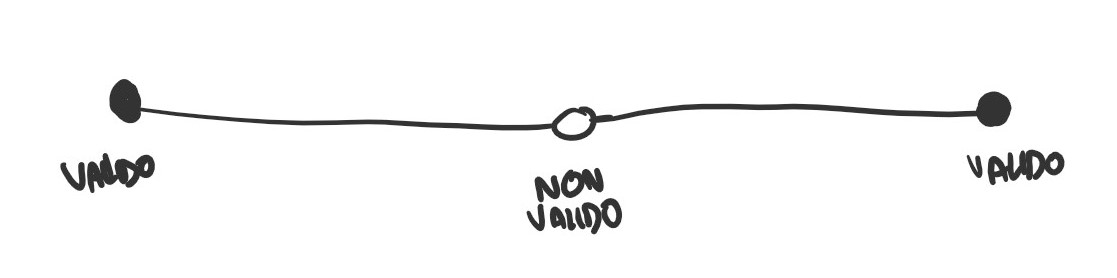
\includegraphics[width=0.7\linewidth]{immagini/img9}
\end{figure}
Nel caso di errore singolo, il messaggio inviato si "sposterebbe" in un vertice adiacente (quindi con distanza di Hamming = 1) che però non verrà accettato dal mittente (visto che i validi sono a distanza 2).

E per quanto riguarda distanza di Hamming = 3?

\begin{figure}[H]
	\centering
	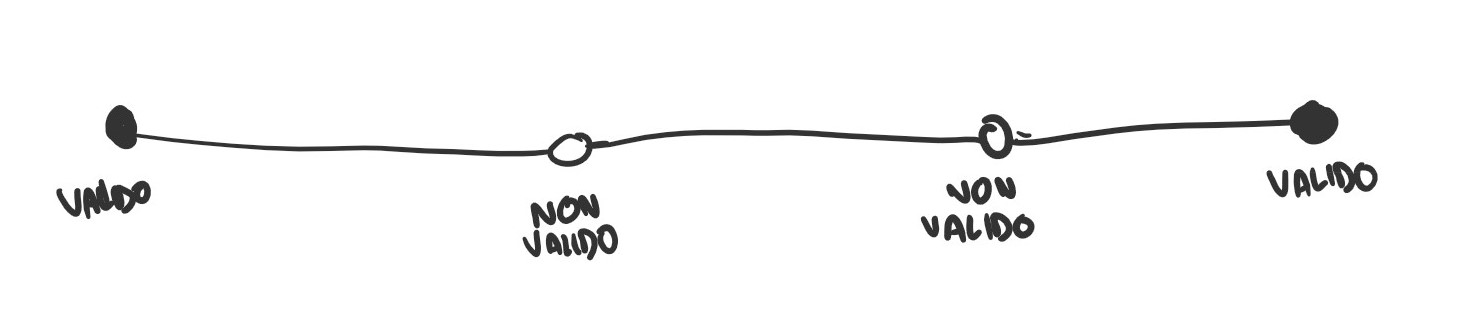
\includegraphics[width=0.7\linewidth]{immagini/img10}
\end{figure}

Nel caso di errore singolo, ci si sposterebbe in questo modo:

\begin{figure}[H]
	\centering
	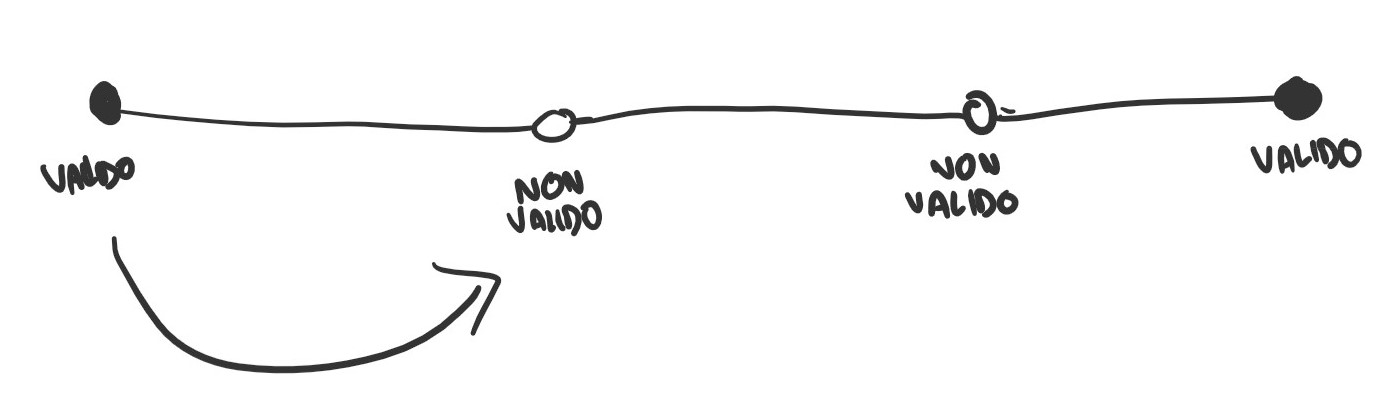
\includegraphics[width=0.7\linewidth]{immagini/img11}
\end{figure}

A questo punto il mittente si chiede: è più probabile che il messaggio arrivi dal vertice a sinistra (con un errore) o dal vertice di destra (con due errori)? Ovviamente è più probabile il vertice sinistro, quindi con questa distanza posso rilevare l'errore e anche correggerlo.
Nel caso di due errori, però, il ricevente sbaglierebbe a correggere l'errore; seguendo l'esempio precedente andrebbe al vertice destro.

Vediamo quindi anche il caso di distanza di Hamming = 4:

\begin{figure}[H]
	\centering
	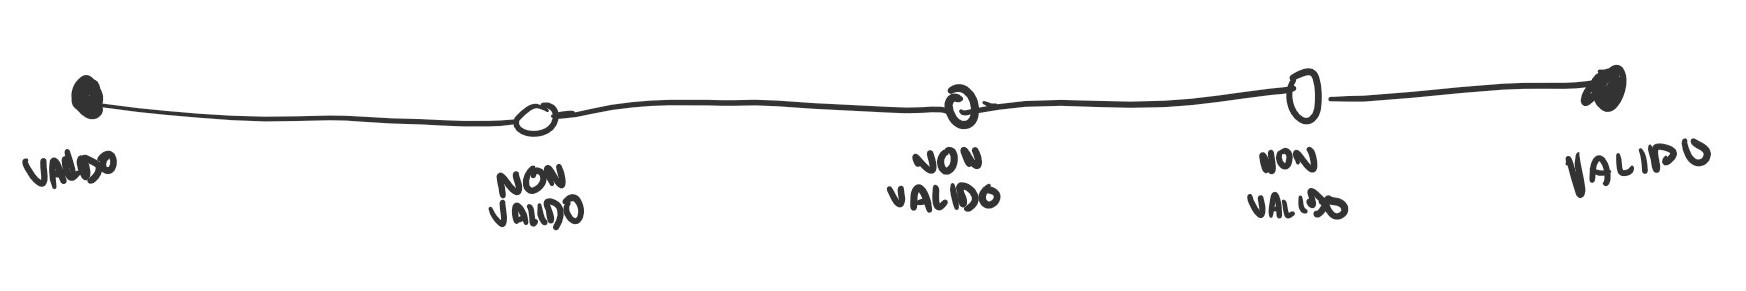
\includegraphics[width=0.7\linewidth]{immagini/img12}
\end{figure}

\'E facile notare come si può correggere facilmente un errore, ma in caso di errore doppio ci si troverà ad un punto equidistante dai due estremi (ovviamente nel caso di tre errori se ne introdurrà un quarto correggendo in maniera sbagliata).

E così via, riassumiamo il tutto con questa tabella:

\begin{table}[h]
	\centering
	\begin{tabular}{l|l|l}
		$d_H$ & errori rilevati & errori corretti \\
		\hline
		1     & 0               & 0               \\
		2     & 1               & 0               \\
		3     & 1               & 1               \\
		4     & 2               & 1               \\
		5     & 2               & 2              \\
		\vdots & \vdots & \vdots
	\end{tabular}
\end{table}

\newpage

\subsubsection*{Sfere}
\addcontentsline{toc}{subsubsection}{Sfere}
Proviamo a cambiare punto di vista, riprendiamo la rappresentazione su segmenti:

%dis

Immaginiamo che il messaggio valido inserito nel canale sia il centro di una sfera.
Se il messaggio che esce fa parte di un unica sfera, lo si può correggere "riportandolo" al centro della sfera. Se invece il messaggio fa parte di più sfere, rilevo l'errore ma non so a quale centro appartenga.

%disegni esempi

Ma come definisco una sfera nello spazio vettoriale? Dico che la sfera \textit{S} è
\begin{equation}
S(x,r) = \{y \in \{0,1\}^n | d_H(x,y) \leq r \}
\end{equation}

Possiamo vedere l'effetto degli errori come una somma xor:

\begin{equation*}
(1,1,0) \oplus (0,1,0) = (1,0,0)
\end{equation*}

In questo caso è avvenuto un posizione 2, quindi è come sommare un vettore con un 1 in posizione 2.

Se capissi qual è il vettore errore mi basterebbe ri-sommarla, per ottenere il messaggio di partenza:

\begin{equation*}
(1,1,0) \oplus (0,1,0) = (1,0,0)
\end{equation*}
\begin{equation*}
(1,0,0) \oplus (0,1,0) = (1,1,0)
\end{equation*}

Riconsideriamo i codici di Hamming con distanza 3, quindi a rilevamento e correzione d'errore singolo.
Ci chiediamo quanto vale il volume della sfera centrata nel vettore che inviamo di raggio 1.

\begin{equation}
V(S(x,1))=1+n
\end{equation}

In generale:

\begin{equation*}
V(S(x,r))=1+n+\binom{n}{2} + \binom{n}{3} + \dots \binom{n}{r}
\end{equation*}
\begin{equation}
V(S(x,r))= \sum_{i=0}^r \binom{n}{i}
\end{equation}

Quanti messaggi validi posso creare in questo modo?
Data distanza di Hamming $d_H=3$, messaggi di \textit{n} bit, quindi uno spazio grande $2^n$ e $n$ sfere grandi $(n+1)$, dico che:

\begin{equation}
\frac{\text{volume spazio}}{\text{volume sfera}} \geq \text{numero massimo di sfere / messaggi}
\end{equation}

\newpage

Applicato al nostro esempio:

\begin{equation*}
\frac{2^n}{n+1} \geq 2^k \; \; \; \; \; \; \; n = k + m
\end{equation*}
\begin{equation*}
2^n \geq 2^k(n+1)
\end{equation*}
\begin{equation*}
\cancel{2^k} 2^m \geq \cancel{2^k}(n+1)
\end{equation*}
\begin{equation*}
2^m \geq n+1
\end{equation*}
Che è la stessa conclusione a cui è arrivato Hamming per i codici ottimali!

\subsection*{Codifica di sorgente}
\addcontentsline{toc}{subsection}{Codifica di sorgente}

L'obiettivo della codifica di sorgente è quello di creare delle codeword ottimali, ad esempio codificando con codeword più piccole i caratteri più utilizzati (codice morse).

Ci sono diversi codici per la codifica di sorgente, distinguibili in due:
\begin{itemize}
	\item Codici a blocchi: tutte le codeword hanno la stessa lunghezza ($\ell_1 = \ell_2 = ... = \ell_q$)
	\begin{itemize}
		\item Vantaggi: il ricevente ha 'vita facile' per decodificare in quanto sa subito quando inizia e quando finisce la codeword (sa già la lunghezza)
		\item Svantaggi: se un simbolo esce con probabilità alta, allora abbiamo un grande spreco (uso gli stessi bit che userei con un simbolo usato raramente)
	\end{itemize}
La lunghezza media delle codeword ($\sum_{i=1}^qp_i = 1$) è ovviamente:
\begin{equation}
L=\sum_{i=1}^q+p_i\ell_i = \sum_{i=1}^qp_i\ell = \ell \sum_{i=1}^qp_i = \ell
\end{equation}
uguale per tutti.
Questo tipo di codice conviene quando la distribuzione delle probabilità per i simboli di uscire è uniforme.
\item Lunghezza variabile: le codeword hanno lunghezze diverse, di solito i caratteri che escono con probabilità $p_i$ maggiori sono codificati in codeword più brevi. 
\begin{itemize}
	\item Vantaggi: C'è meno spreco di spazio, le codeword si adattano alle probabilità dei simboli
	\item Svantaggi: Per il ricevente non è semplice capire quando una codeword finisce.
\end{itemize}
A causa di questo svantaggio si introducono due sottoclassi dei codici a lunghezza variabile:
\begin{itemize}
	\item Univocamente decodificabili: quando il ricevente riceve una sequenza di codeword (es $w_1, w_2 \dots w_k$) di lunghezza diversa, allora esiste un unico modo di spezzare la sequenza di codeword
	\item Non univocamente decodificabili: al contrario, non esiste un unico modo di spezzare la sequenza ricevuta (ad esempio posso spezzare una sequenza sia in $s_1s_1s_2$ che in $s_3s_2$).
\end{itemize}
Nel corso useremo \textbf{solo} codici univocamente decodificabili.
\end{itemize}









